\subsubsection{Microcontrolador y placa STM32 Nucleo-144}

El procesamiento central del sistema se realiza en el microcontrolador STM32F429ZI incluido en la placa STM32 Nucleo-144. La placa permite la alimentación del MCU y de todos sus circuitos a través de distintas entradas como se puede observar en la figura \ref{fig:nucleo_pw}. Para el SAL/T, se utilizó la entrada de E5V para alimentar la placa utilizando la fuente de alimentación del sistema y para eso se debe colocar en el JP3 un cortocircuito entre los pines 1 y 2 para tomar la tensión de allí. Se observa que la placa incluye un circuito de regulación de tensión a 3V3 para alimentar el MCU y otros circuitos internos. 


\begin{figure}[H]
    \centering
    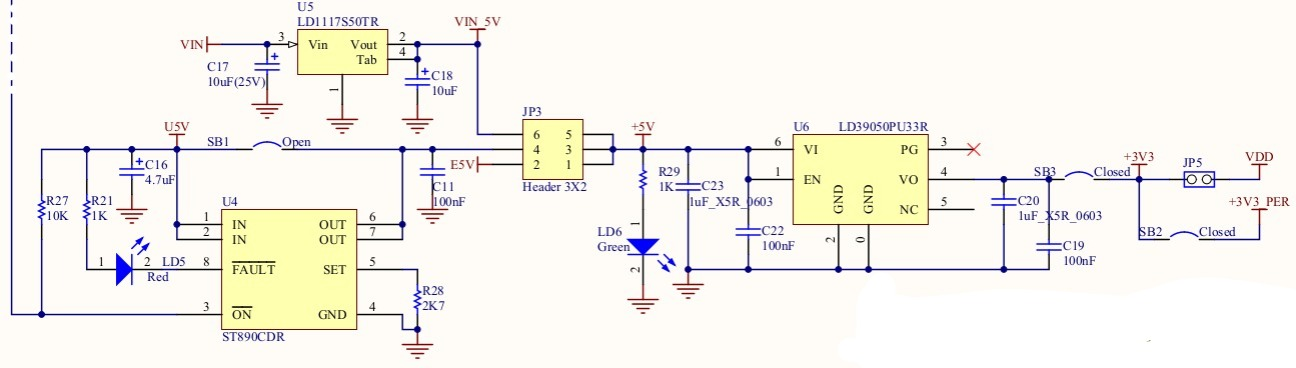
\includegraphics[width = \linewidth]{img/nucleo_pw.jpeg}
    \caption{Esquemático de la alimentación de la placa STM32 Nucleo-144}
    \label{fig:nucleo_pw}
\end{figure}    

Para la inserción de la STM32 Nucleo-144 en la placa principal del SAL/T, se utilizaron los conectores de expansión morpho que permiten el acceso a todos los pines del MCU al usuario. Para eso, se soldaron los pines en la Nucleo y se colocaron conectores hembra en la placa principal. Se necesitaron 2 conectores de 2x36 pines cada uno para conectar la placa. Este tipo de conectores permite colocar y sacar la placa fácilmente lo que permite manipularla mejor para la programación y cualquier prueba de circuitos que se quiera realizar sin la placa colocada. En la figura \ref{fig:diagrama_bloques_coms} se mostraron las distintas interfaces utilizadas del microcontrolador en las que se incluye ADC, SPI, UART, I2C y GPIO. 